\documentclass[handout]{beamer}

\input{../Vor2017glærur}

\title{Tölvunarfræði 2}
\subtitle{Vika 5}

\begin{document}

\begin{frame}
\titlepage
\end{frame}

\section{Inngangur}

\begin{frame}{Í dag}
\begin{itemize}
 \item Skoðum þrjár hugrænar gagnagerðir
 \begin{itemize}
  \item Skjóðu \eng{bag}
  \item Biðröð \eng{queue}
  \item Hlaða \eng{stack}
 \end{itemize}
 \item Koma fyrir í fjölmörgum þekktum reikniritum
 \item Getum notað þær til að skilgreina flóknari hugrænar gagnagerðir
\end{itemize}
\end{frame}

\section{Skjóður}

\begin{frame}{Skjóður}
\begin{itemize}
 \item Við notum skjóður til að geyma ``hluti''
 \item Til að hægt sé að tala um skjóðu þurfum við að geta sett nýja hluti í skjóðuna og skoðað gögnin sem eru í henni
 \item Skjóða þarf ekki að styðja eyðingu
 \begin{itemize}
  \item Einföld gagnagerð, getum notað hana þegar þarfir okkar eru einfaldar
 \end{itemize}
 \item Við þurfum að geta ítrað yfir gögn skjóðunnar á skilvirkan hátt
\end{itemize}
\end{frame}

\begin{frame}{API}
Bókin skilgreinir skil sem eru viðeigandi fyrir útfærslu á skjóðu í Java:
\begin{center}
\begin{tabular}{rll}
\toprule
\multicolumn{3}{c}{\texttt{public class Bag<Item> implements Iterable<item>}}\\
\midrule
-&\texttt{Bag()}& Smiður, býr til tóma skjóðu\\
\texttt{void}&\texttt{add(Item item)}&Bæta \texttt{item} við skjóðuna\\
\texttt{boolean}&\texttt{isEmpty()}&Er skjóðan tóm?\\
\texttt{int}&\texttt{size()}&Fjöldi hluta í skjóðunni\\
\bottomrule
\end{tabular}
\end{center}
\end{frame}

\subsection{Iterable}

\begin{frame}[fragile]{Iterable?}
\begin{columns}
\column{0.5\textwidth}
\begin{itemize}
 \item Java hefur innbyggðan stuðning fyrir ``interfaces'' (ísl. \emph{skil}? \emph{Viðmót}?)
 \item Getum sagt að klasi \texttt{A} eigi að útfæra skil \texttt{B} með
 \begin{minted}{java}
 class A implements B
 \end{minted}
 \item Þetta felur í sér loforð um að \texttt{A} muni uppfylla skilin \texttt{B}
\end{itemize}
\column{0.5\textwidth}
\href{https://docs.oracle.com/javase/8/docs/api/java/lang/Iterable.html}{\texttt{Iterable}} eru sérstök skil í Java-málinu sem gera það mögulegt að nota ``foreach'' lykkjur á tilvik klasa sem uppfylla þau
\begin{minted}{java}
// List uppfyllir Iterable
List<T> list = ... 
for (T item : list) {
 ... // Vinna með item
}
\end{minted}
\end{columns}
\end{frame}

\begin{frame}{Að uppfylla Iterable}
\begin{columns}
\column{0.5\textwidth}
\begin{itemize}
 \item Hvað gerist í foreach lykkju?
 \begin{itemize}
  \item Búið er til tilvik af ítrara 
  \item Athugað ítrarinn \texttt{hasNext()}
  \item Ef ítrarinn \texttt{hasNext()}, framkvæma \texttt{getNext()}
 \end{itemize}
 \item Þetta fer fram ``bak við tjöldin'' ef viðkomandi klasi uppfyllir \texttt{Iterable}
\end{itemize}
\column{0.5\textwidth}
\begin{itemize}
 \item Til að uppfylla \texttt{Iterable} þurfum við að skrifa aðgerðina \texttt{iterator()} sem skilar ítrara
 \item Í Java er ítrari klasi sem uppfyllir \href{https://docs.oracle.com/javase/8/docs/api/java/util/Iterator.html}{\texttt{Iterator}}
 \item Skoðum \texttt{Bag.java} (af Algs4 síðunni)
\end{itemize}
\end{columns}
\end{frame}

\section{Hlaðar}

\begin{frame}{Hlaðar}
\begin{columns}[c]
\column{0.5\textwidth}
\begin{itemize}
 \item Hlaði er hugræn gagnagerð
 \item Getum sett stök á hlaða og fjarlægt þau þaðan aftur
 \item Röðin er skilgreinandi fyrir hlaða - hlaði skal vera ``Last-in, first-out'' (LIFO)
\end{itemize}
\column{0.5\textwidth}
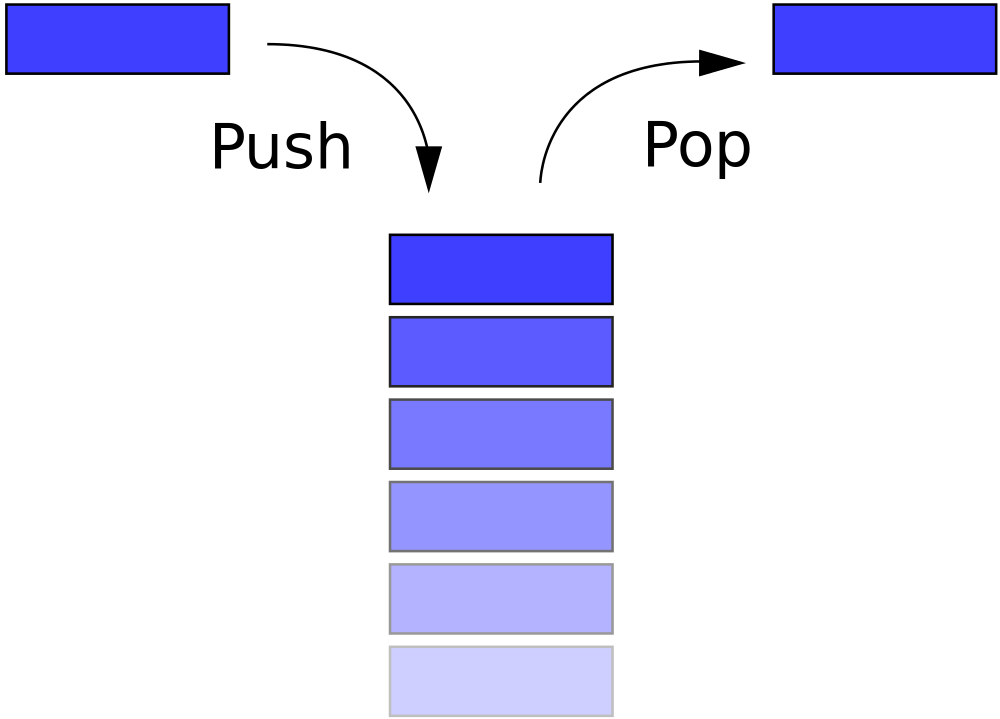
\includegraphics[width=\linewidth]{Pics/stack}
\end{columns}
\end{frame}

\begin{frame}{API}
\begin{center}
\begin{tabularx}{\textwidth}{rlX}
\toprule
\multicolumn{3}{c}{\texttt{public class Stack<Item> implements Iterable<item>}}\\
\midrule
-&\texttt{Stack()}& Smiður, býr til tóman hlaða\\
\texttt{void}&\texttt{push(Item item)}&Bæta \texttt{item} á hlaðann\\
\texttt{Item}&\texttt{pop()}&Fjarlægja og skila því staki sem styst hefur verið á hlaðanum\\
\texttt{boolean}&\texttt{isEmpty()}&Er hlaðinn tómur?\\
\texttt{int}&\texttt{size()}&Fjöldi hluta á hlaðanum\\
\bottomrule
\end{tabularx}
\end{center}
\end{frame}

\begin{frame}{Hlaðar}
\begin{itemize}
 \item Hugmyndir tengdar hlöðum koma mjög víða við
 \begin{itemize}
  \item Geymsla á sögu í vafra
  \begin{itemize}
   \item Það að smella á tengil setur síðu á hlaða, það að smella á ``back'' takkann 
  \end{itemize}
 \item Geymsla á sögu fallskalla í forriti
  \begin{itemize}
   \item Höfum kynnst þessu sem ``hlaðanum'' í C++
  \end{itemize}
 \item Alls kyns reiknirit
 \begin{itemize}
  \item Útreikningur á reiknisegðum
  \item Skoðum \texttt{Evaluate.java}
 \end{itemize}
 \end{itemize}
\end{itemize}
\end{frame}

\section{Biðraðir}

\begin{frame}{Biðraðir}
\begin{columns}[c]
\column{0.5\textwidth}
\begin{itemize}
 \item Biðröð er hugræn gagnagerð
 \item Getum sett stök í biðröð og fjarlægt þau aftur
 \item Röðin er skilgreinandi fyrir biðröð - biðröð skal vera ``First-in, first-out'' (FIFO) 
\end{itemize}
\column{0.5\textwidth}
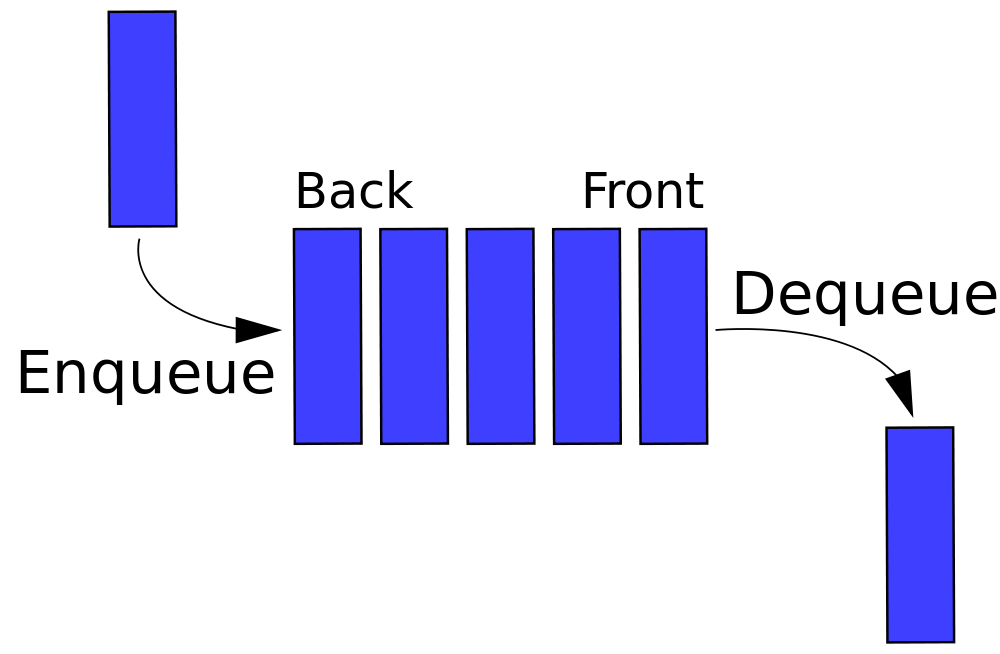
\includegraphics[width=\linewidth]{Pics/queue}
\end{columns}
\end{frame}

\begin{frame}{API}
\begin{center}
\begin{tabularx}{\textwidth}{rlX}
\toprule
\multicolumn{3}{c}{\texttt{public class Queue<Item> implements Iterable<Item>}}\\
\midrule
-&\texttt{Queue()}& Smiður, býr til tóma biðröð\\
\texttt{void}&\texttt{enqueue(Item item)}&Bæta \texttt{item} við biðröðina\\
\texttt{Item}&\texttt{dequeue()}&Fjarlægja og skila því staki sem lengst hefur verið í biðröðinni\\
\texttt{boolean}&\texttt{isEmpty()}&Er biðröðin tóm?\\
\texttt{int}&\texttt{size()}&Fjöldi hluta í biðröðinni\\
\bottomrule
\end{tabularx}
\end{center}
\end{frame}

\begin{frame}{Biðraðir}
\begin{itemize}
 \item Biðraðir koma við sögu í ýmsum samhengjum þar sem búist er við ``sanngirni''
 \begin{itemize}
  \item Einföld tímaniðurröðunarreiknirit í stýrikerfum
  \item Getum sett upplýsingar sem tengjast raunverulegum hlutum í biðröð
 \end{itemize}
 \item Hjálpargagnagrind í ýmsum reikniritum
 \begin{itemize}
  \item Dæmi: Breiddarleit í neti
 \end{itemize}
\end{itemize}
\end{frame}

\section{Greining reiknirita}

\begin{frame}{Keyrslutími}
\begin{itemize}
 \item Möguleg leið til að athuga hvort forrit séu ``hröð'' - nota skeiðklukku
 \begin{itemize}
  \item \href{http://algs4.cs.princeton.edu/code/edu/princeton/cs/algs4/Stopwatch.java.html}{Stopwatch.java}
 \end{itemize}
 \item Meiri/önnur innsýn fæst samt oft með því að
 \begin{enumerate}
  \item Athuga hve lengi hver skipun í forritunarmálinu tekur
  \item Telja hve oft hver skipun kemur fyrir
 \end{enumerate}
\end{itemize}
\end{frame}

\begin{frame}{Stærð inntaks og keyrslutími}
\begin{itemize}
 \item Reiknirit sem við skoðum vinna oft á gögnum af breytilegri stærð
 \item Við getum mjög oft lýst stærð inntaks með afstæðum hætti
 \begin{itemize}
  \item Klassískt tákn: $n$
  \item $n$ getur verið fjöldi hnúta í lista, fjöldi lína í bók, fjöldi tákna í streng\ldots
 \end{itemize}
 \item Lýsum keyrslutímanum sem falli af inntaksstærðinni
 \begin{itemize}
  \item Dæmi: Keyrslutími aðferðar getur verið $n(n-1)(n-2)/6$
 \end{itemize}
\end{itemize}
\end{frame}

\begin{frame}{Einföldun}
Keyrslutími á ``litlum'' inntökum er venjulega hverfandi, meira púður fer í að skoða hegðun á stórum skala. Bókarhöfundar nota slöngunálgun \eng{tilde approximation} til að einfalda framsetningu.
\begin{tcolorbox}
Við skrifum $g(n) \sim f(n)$ þegar $\frac{g(n)}{f(n)}$ stefnir á 1 þegar $n$ vex.
\end{tcolorbox}
Þá getum við skrifað $n(n-1)(n-2)/6 \sim \frac{n^3}{6}$ og sagt að keyrslutími aðferðar með nákvæman keyrslutíma $n(n-1)(n-2)/6$ sé $\sim \frac{n^3}{6}$.

\vspace{1cm}
Mjög svipuð hugtök: Stóra-$O$ og stóra-$\Theta$-rithættir.
\end{frame}

\section{Lokaorð}

\begin{frame}{Þessi glærupakki}
Tengill á fyrirlestraræfingu: \url{https://goo.gl/forms/fH4spAHQlQX8vIkB2}
\vspace{1cm}

\texttt{Evaluate.java} má finna á \href{https://github.com/Ernir/kennsluefni/tree/master/T2/Code/w4}{Github}. 

Kóða fyrir \texttt{Bag}, \texttt{Stack} og \texttt{Queue} má finna á \url{http://algs4.cs.princeton.edu/code/}
\end{frame}

\begin{frame}{Næst}
Röðun
\end{frame}


\end{document}
